\appendix

\section{Additional Implementation Details}
As indicated in the manuscript, we adopted CLIP ViT-B/16 as our encoders.
Yet, since the image encoder was trained with images of 224x224 resolution, we resized the position embeddings of the image encoder to adapt CLIP to handle the images of 384x384 resolution.
For $\phi_c(\cdot)$ that projects semantic vectors for SPT, we share one linear layer across all visual encoder layers of CLIP.
Also, $M$, the number of learnable tokens in SPT is designated to 10.
For LAT, the learnable matrices $W$ and $B$ are initialized to 1 and 0, respectively, and the thresholds for the rank-contrastive loss are set to [0.8, 0.6, 0.4], establishing the iteration count $K$ to 3.
Finally, for SaSC, we extract encoder feature $\mathcal{V}$ from layers $l = [7,8,9]$, and pass onto the decoder feature $\mathcal{F}$ at layers $k = [2,3,4]$.


\section{Effect of Learnable Tokens}

\subsection{Effect of the Number}
We determine the optimal number of learnable tokens required to facilitate an effective transfer of CLIP.
An extremely small number of learnable tokens might not be sufficient to effectively facilitate the transfer of a pre-trained large model.
However, employing an excessive number of visual prompts also can have a detrimental impact on our model's performance due to the loss of generality of CLIP.
Based on experiments as reported in Fig.~\ref{fig:num}, we have determined that the optimal number of learnable tokens for our specific task is 10.

\subsection{Effect of the Depth}
In addition to the apparent influence of the number of learnable tokens on ZSOC performance, we also anticipate that the specific placement of these tokens within the encoder layers will have a substantial impact.
To provide clearer context, we assign numerical labels to the 12 layers of the vision transformer in the CLIP image encoder, ranging from 1 to 12.
We observe that introducing prompt tokens on the earlier layers typically results in improved performance compared to placement on the latter layers as reported in Tab.~\ref{tab:depth}.
The highest performance is achieved when learnable prompt tokens are inserted into every image encoding layer~(layer 1--12), which also serves as the default setting in our experimental setup.


\begin{figure}[ht]
    \begin{center}
    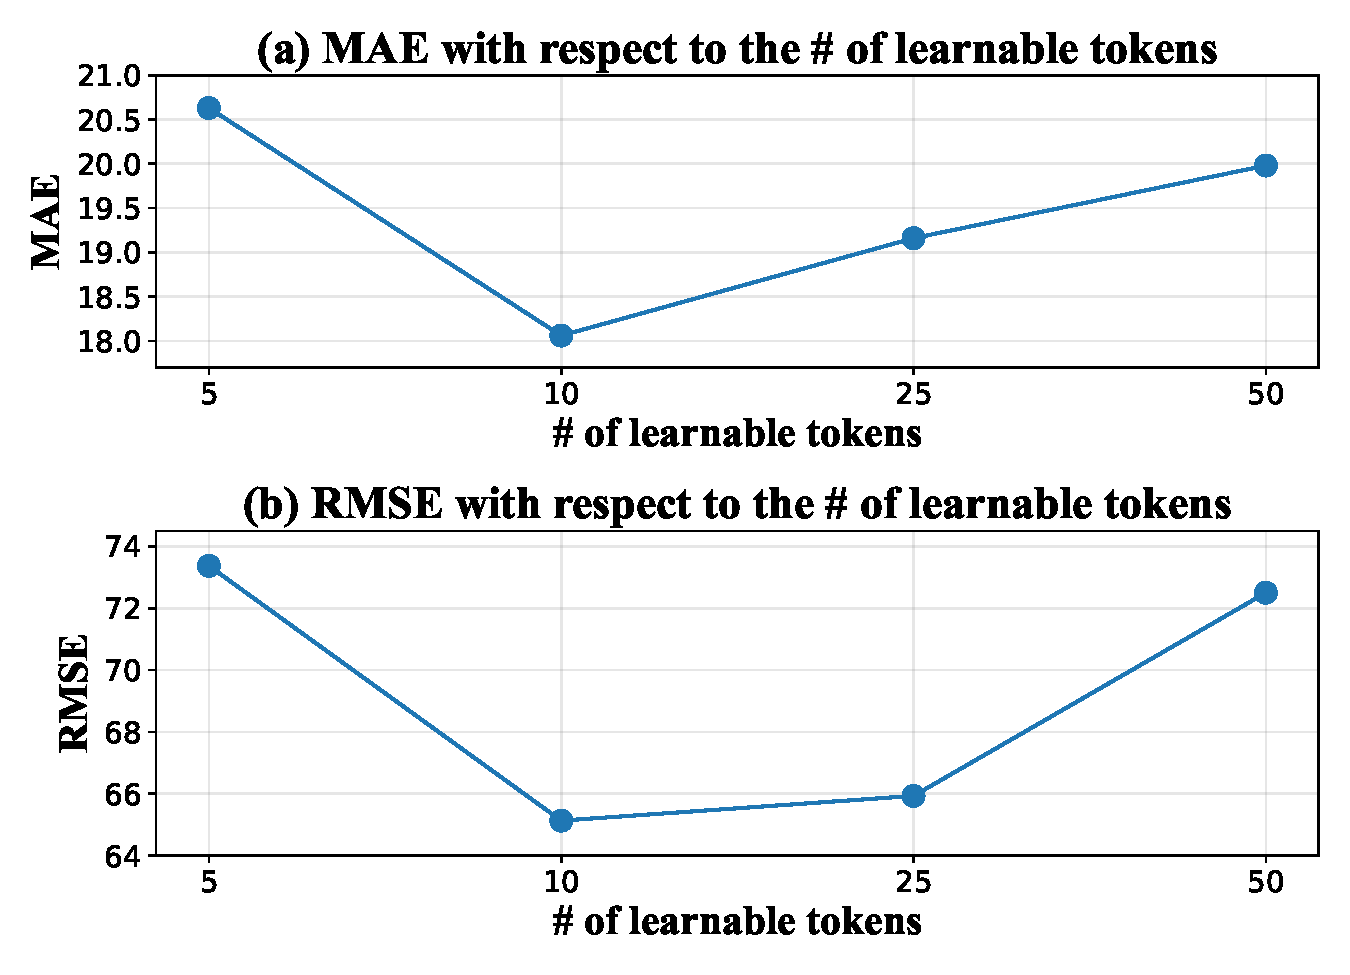
\includegraphics[width=\linewidth]{figs/SPT_ablation.pdf}
    \end{center}
    \caption{
        Effect of the number of learnable tokens.
    }
    \label{fig:num}
\end{figure}

\begin{table}[h]
    \small
    \setlength{\extrarowheight}{2.3pt}
    \setlength{\tabcolsep}{1.5pt}
    \centering
    \begin{tabular*}{\linewidth}{l@{\extracolsep{\fill}}*{5}{c}}
    \hline
    \multicolumn{2}{c}{\multirow{2}{*}{Condition}} & \multicolumn{2}{c}{Val set} & \multicolumn{2}{c}{Test set} \\
    \cline{3-4}\cline{5-6}
     & & MAE & RMSE & MAE & RMSE \\
    \hline
    \multicolumn{2}{c}{1 -- 3} & 20.5 & 68.81 &	19.73 & 111.6 \\
    \multicolumn{2}{c}{1 -- 6} & 19.72 & 66.70 & 20.23 & \textbf{103.44} \\
    \multicolumn{2}{c}{10 -- 12} & 23.34 &	81.39 &	21.81 &	110.92 \\
    \multicolumn{2}{c}{7 -- 12} & 23.32 &	80.05 &	22.16 &	105.42 \\
    \multicolumn{2}{c}{1 -- 12} & \textbf{18.06} & \textbf{65.13} & \textbf{17.05} & 106.16 \\ 
    \hline
    % \hline
    \end{tabular*}
    \caption{Effect of the depth of learnable tokens}
    \label{tab:depth}
\end{table}


\section{LAT Value Distribution}
In our manuscript, we mentioned that LAT is to facilitate the conversion of similarity maps to be more counting-specific: guiding activations to be more compact on object centers and not significantly modifying the similarity map.
To substantiate our argument, we plot the distributions of $W$ and $B$ matrices in Fig.~\ref{fig:LAT}.
As we observe that the values of $W$ and $B$ are concentrated around 1 and 0, respectively, we confirm that LAT maintains the localization capability of our encoder and only fine-tunes the similarity map to be more counting-specific.

\begin{figure}[ht]
    \begin{center}
    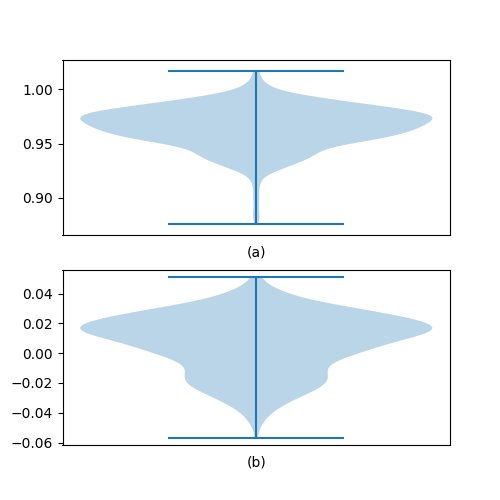
\includegraphics[width=\linewidth]{figs/LAT.png}

    \end{center}
    \caption{
        (a) displays a distribution diagram of the values in $W$, while (b) illustrates the distribution of values in $B$, both of which are employed for the affine transformation of LAT.
    }
    \label{fig:LAT}
\end{figure}

\section{Effect of Encoder Features in SaSC}
Building upon the arguments presented in SaSC, which emphasize the attainment of generalizability and rich semantics through the aggregation of encoder features during decoding, we explore the combinations of the successive layers to yield the best results.
Through this investigation, we aim to determine which layer's features are most conducive to enhancing the overall performance of the decoding process.
\begin{figure}[ht]
    \begin{center}
    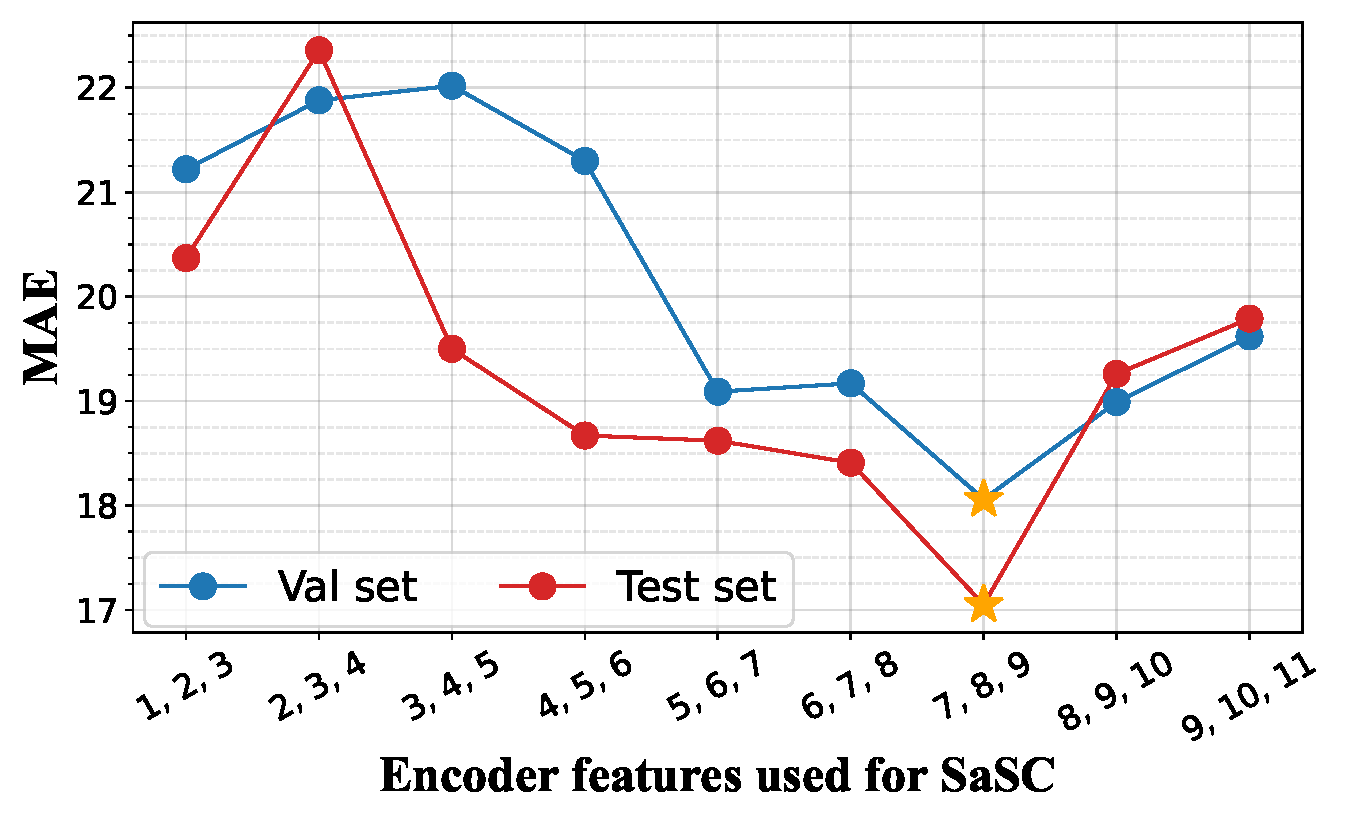
\includegraphics[width=\linewidth]{figs/SaSC_ablation.pdf}
    \end{center}
    \caption{
        Effect of the combinations of encoder layers.
    }
    \label{fig:sasc}
\end{figure}

Evidently, Fig.~\ref{fig:sasc} shows that the shallow encoder layers do not perform well due to their limited acquisition of meaningful patch-level information.
In addition, we find a similar tendency to the arguments presented by \cite{li2023clipsurgery}, mentioning that  Feed Forward Networks~(FFNs) in the deeper CLIP layers are more likely to bring negative impacts on the vision-language alignment and localization capabilities.
In this context, we have chosen the features from the 7th, 8th, and 9th encoding layers and incorporated them into the 2nd, 3rd, and 4th decoding layers.

\section{Context Prompts}
In Tab.~5 in our manuscript, we demonstrated the influence of the form of context prompts.
Here, we provide the lists of prompts that were used for the experiments.

For singular form, below 15 templates were used:\newline
'A photo of a \{\}.',\newline
'A photo of a small \{\}.',\newline
'A photo of a medium \{\}.',\newline
'A photo of a large \{\}.',\newline
'This is a photo of a \{\}.',\newline
'This is a photo of a small \{\}.',\newline
'This is a photo of a medium \{\}.',\newline
'This is a photo of a large \{\}.',\newline
'A \{\} in the scene.',\newline
'A photo of a \{\} in the scene.',\newline
'There is a \{\} in the scene.',\newline
'There is the \{\} in the scene.',\newline
'This is a \{\} in the scene.',\newline
'This is the \{\} in the scene.',\newline
'This is one \{\} in the scene.',\newline

For plural form, below 11 templates were used:\newline
'A photo of a number of \{\}.'\newline
'A photo of a number of small \{\}.'\newline
'A photo of a number of medium \{\}.'\newline
'A photo of a number of large \{\}.'\newline
'There is a photo of a number of \{\}.'\newline
'There is a photo of a number of small \{\}.'\newline
'There is a photo of a number of medium \{\}.'\newline
'There is a photo of a number of large \{\}.'\newline
'A number of \{\} in the scene.'\newline
'A photo of a number of \{\} in the scene.'\newline
'There are a number of \{\} in the scene.'\newline

\section{Additional Qualitative Results}
In addition to qualitative results in the manuscript, we provide more results in Fig.~\ref{fig:qualitative_results_suppl}, comparing the vision-language similarity map and the density map produced by our VLBase and VLCounter on the FSC147 dataset.
Note that we could not compare with the previous two-stage baselines since their implementations are not fully publicized.

% 정성 평가 결과 그림
\begin{figure*}[t]
    \begin{center}
        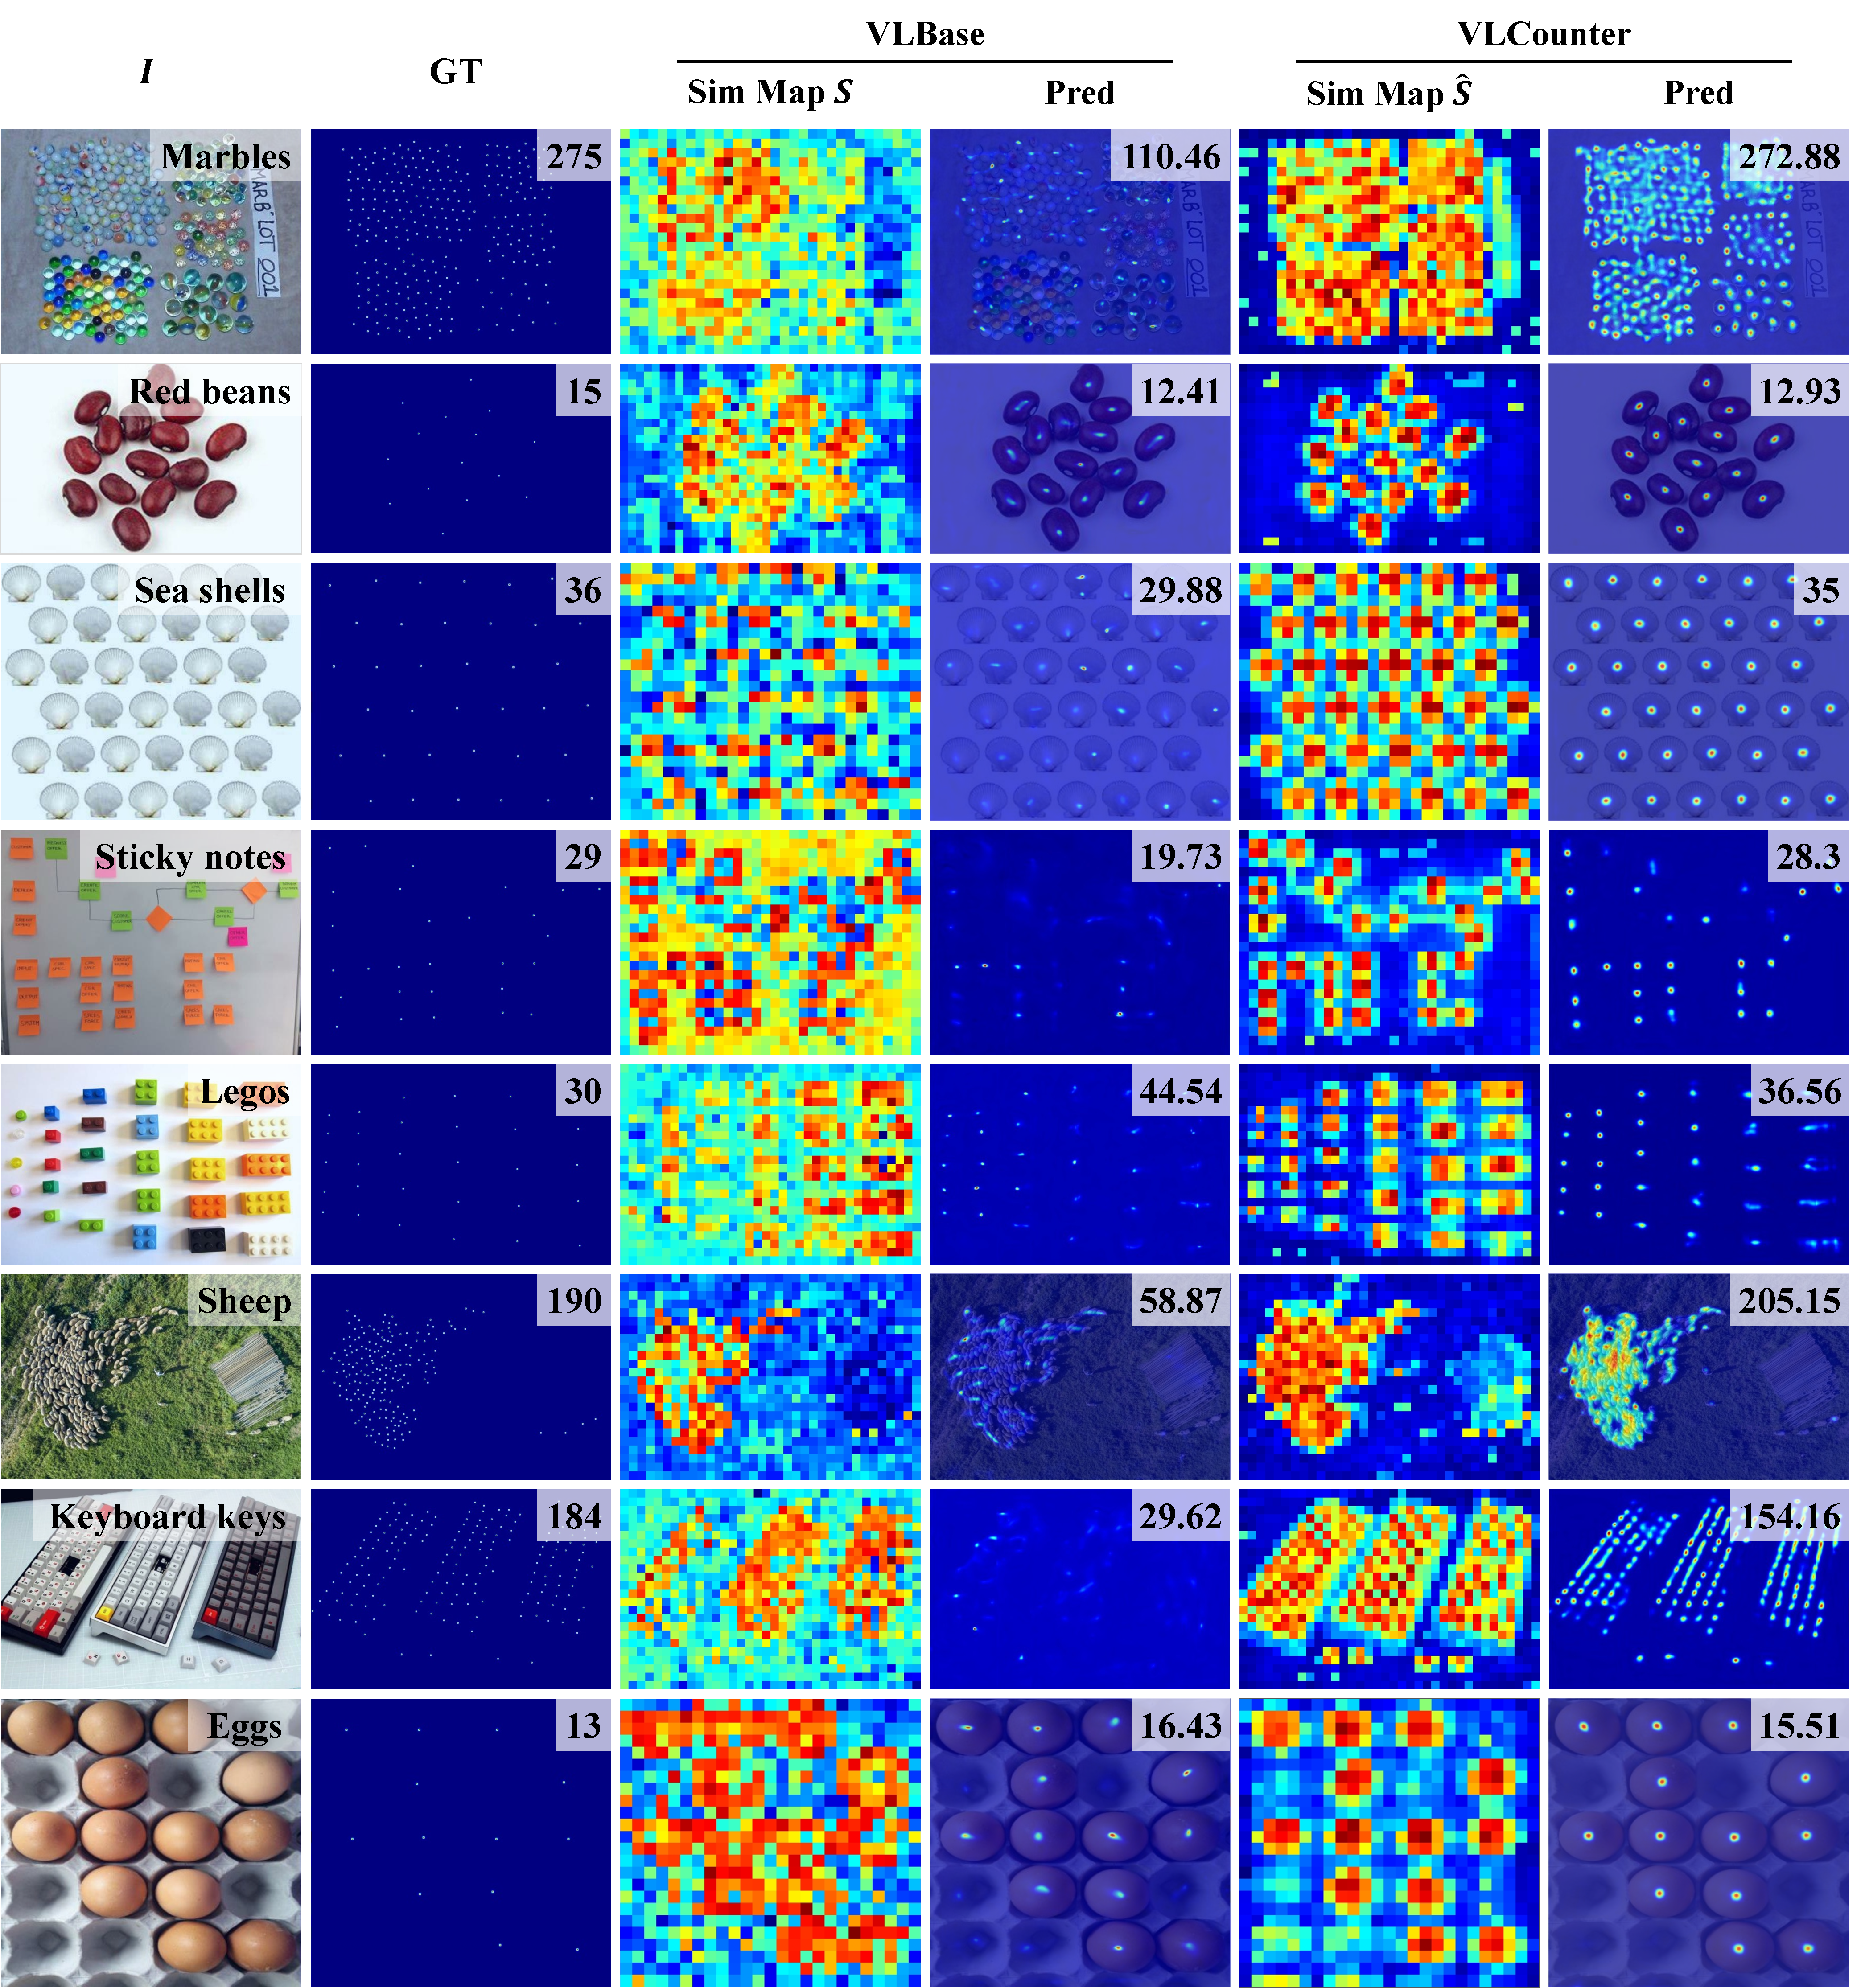
\includegraphics[width=\linewidth]{figs/qualitative_suppl.pdf}
    \end{center}
    \caption{
        Qualitative comparison of VLBase and VLCounter on the FSC-147.
        Class names and counting values are shown at the right top of the query image~($I$) and the predicted density map, respectively.
    }
    \label{fig:qualitative_results_suppl}
\end{figure*}

\section{Comparison to Concurrent Work}
Recently, many efforts have been made to perform pixel-level dense prediction using CLIP.
While a concurrent work, CLIP-count~\cite{jiang2023clip}, requires additional parameters for visual-text interaction layers, we point out that our approach does not charge much memory cost since we leverage the semantic tokens within the image encoding process.
In Tab.~\ref{tab:clipcount}, we compare the number of learnable parameters and Multiply–ACcumulate~(MACs), revealing that our method shows an advantage in computational efficiency.
Moreover, while our performances seem to bring marginal benefits over CLIP-Count on the FSC-147 dataset~(Tab.~\ref{tab:clipcount_fsc}), we emphasize the large performance gaps in cross-domain scenarios in Tab.~\ref{tab:clipcount}~(+44.4\% and +5\% on CARPK and IOCfish5k datasets in MAE, respectively).

\begin{table}[h]
    \small
    \setlength{\extrarowheight}{2.3pt}
    \setlength{\tabcolsep}{1.5pt}
    \centering
    \begin{tabular*}{\linewidth}{l@{\extracolsep{\fill}}*{5}{c}}
    \hline
    \multicolumn{2}{c}{\multirow{2}{*}{Methods}} & \multicolumn{2}{c}{Val set} & \multicolumn{2}{c}{Test set} \\
    \cline{3-4}\cline{5-6}
     & & MAE & RMSE & MAE & RMSE \\
    \hline
    \multicolumn{2}{c}{CLIP-Count} & 18.76 & \textbf{61.18} & 17.78 & 106.62 \\
    \multicolumn{2}{c}{VLCounter~(Ours)} & \textbf{18.06} & 65.13 & \textbf{17.05} & \textbf{106.16} \\
    \hline
    % \hline
    \end{tabular*}
    \caption{Comparision with CLIP-Count on FSC147 dataset}
    \label{tab:clipcount_fsc}
\end{table}

\begin{table*}[t!]
    \small
    \setlength{\extrarowheight}{1.8pt}
    % \setlength{\tabcolsep}{5pt}
    \centering
    % \begin{tabular}{ccccccc}
    \begin{tabular*}{\textwidth}{@{\extracolsep{\fill}}*{7}{c}}
    \hline
    Methods & Learnable Params~(M) & MACs~(G) & CARPK~(MAE) & CARPK~(RMSE) & IOCfish5k~(MAE) & IOCfish5k~(RMSE) \\
    \hline
    CLIP-Count & 16.36 & 123.06 & 11.70 & 13.94 & 82.1 & 155.2 \\
    \hline
    Ours & \textbf{1.44} & \textbf{34.36} & \textbf{6.46} & \textbf{8.68} & \textbf{78.0} & \textbf{154.9} \\
    \hline
    \end{tabular*}
    \caption{Comparision with CLIP-Count in the number of learnable parameters, MACs, and performance on diverse datasets}
    \label{tab:clipcount}
\end{table*}

